
%(BEGIN_QUESTION)
% Copyright 2012, Tony R. Kuphaldt, released under the Creative Commons Attribution License (v 1.0)
% This means you may do almost anything with this work of mine, so long as you give me proper credit

A ``smart'' (digital) DP pressure transmitter is removed from service and taken to a calibration bench for testing.  A technician connects a precision pressure gauge and air source to the transmitter's high port while monitoring the 4-20 mA output signal using a DMM:

$$\includegraphics[width=15.5cm]{i02033x01.eps}$$

Calculate the amount of {\it sensor trim} error as well as the amount of {\it output trim} error, both expressed in percent of span.  Also, explain why the HART communicator is necessary to be able to separately calculate these error values.

\vskip 20pt \vbox{\hrule \hbox{\strut \vrule{} {\bf Suggestions for Socratic discussion} \vrule} \hrule}

\begin{itemize}
\item{} What other possible sources of error besides the transmitter could account for these discrepancies?
\item{} Suppose another instrument technician suggests to you that a problem within the precision air pressure regulator might account for some (or all!) of the calibration error seen in the data, and that we should replace the regulator with another.  How would you respond to this suggestion?
\item{} Suppose another instrument technician suggests to you that a problem within the loop resistor might account for some (or all!) of the calibration error seen in the data, and that we should replace the resistor with another.  How would you respond to this suggestion?
\item{} Does the HART communicator need to be NIST traceable?  Why or why not?
\end{itemize}

\underbar{file i02033}
%(END_QUESTION)





%(BEGIN_ANSWER)


%(END_ANSWER)





%(BEGIN_NOTES)

$$\hbox{Sensor trim error:} \hskip 20pt \left({28.75 - 28.70 \over 35}\right) 100\% = +0.142857\%$$

$$\hbox{Output trim error:} \hskip 20pt \left({17.53 - 17.14 \over 16}\right) 100\% = +2.4375\%$$


%INDEX% Calibration, smart transmitter: digital trim
%INDEX% Fieldbus, HART: communicator variables
%INDEX% Measurement, pressure: troubleshooting

%(END_NOTES)

